\documentclass[journal,twoside]{IEEEtran}

\usepackage{texnames}
\usepackage{graphicx}
\graphicspath{{../../../Figures/PDF/}{../../../Figures/PNG/}}
\DeclareGraphicsExtensions{.pdf,.png,.jpg,.jpeg}

\usepackage{color}
\usepackage{amsmath}
\interdisplaylinepenalty=2500
\usepackage{algorithmic}
\usepackage{array}
\usepackage[font=footnotesize,margin=1ex]{subcaption}
%\usepackage{dblfloatfix}
\usepackage[binary-units = true]{siunitx}
\usepackage{url}
\usepackage{booktabs}

%\usepackage{tikz}
%\usetikzlibrary{shapes.geometric,arrows,trees}
%
%
%\tikzstyle{root} = [rectangle, rounded corners, minimum width=2cm, minimum height=.7cm, text centered, draw=black, fill=blue!30]
%\tikzstyle{files} = [rectangle, minimum width=1cm, minimum height=.5cm, text centered, draw=black, fill=white]
%\tikzstyle{link} = [thick, -]

\begin{document}
	
\title{Proposal of a Badging System for Reproducibility and Replicability in Remote Sensing Research}
	
\author{Alejandro~C.~Frery,~\IEEEmembership{Senior Member,~IEEE,}
Luis~Gomez,~\IEEEmembership{Senior Member,~IEEE,}
and~Antonio~C.~Medeiros% <-this % stops a space
\thanks{A.\ C.\ Frery and A.\ C.\ Medeiros are with the \textit{Laborat\'orio de Computa\c c\~ao Cient\'ifica e An\'alise Num\'erica} -- LaCCAN, Universidade Federal de Alagoas, Macei\'o, Brazil.
A.\ C.\ Frery is also with the Key Lab of Intelligent Perception and Image Understanding of the Ministry of Education, Xidian University, Xi'an, China. (email: acfrery@laccan.ufal.br)}% <-this % stops a space
\thanks{Luis Gomez is with the Universidad de Las Palmas de Gran Canaria, Spain}% <-this % stops a space
\thanks{Manuscript received XX, accepted YY.}}
	
\markboth{IEEE Journal of Selected Topics on Applied Earth Observations and Remote Sensing,~Vol.~XX, No.~YY, Month~2020}%
{Frery \MakeLowercase{\textit{et al.}}: Badging Reproducibility and Replicability}
	
\maketitle
	
\begin{abstract}
\textcolor{red}{Remote Sensing is a truly active research area, where many actors play a fundamental role, from industry (public or private) to large or small research groups. 
From that intensive activity, methods, algorithms and techniques are continuously published or broadcasted through papers, conferences, repositories or other means. 
In most cases, there is a sound interest from researchers to use those methods, what implies easy availability of the related methods (computational codes or more detailed descriptions) and implicitly, that method have been extensively tested and they are ready for its use. 
Reproducibility research comprises all those issues just mentioned. In this paper, we aim to provide insights to complement the visibility of research in the area of Remote Sensing and, what is considered more relevant: to \textit{seduce} Authors to include those resources  in their common scientific activity.}
\end{abstract}
	
\begin{IEEEkeywords}
Reproducibility,
Replicability,
Remote Sensing
\end{IEEEkeywords}
	

\IEEEpeerreviewmaketitle

\section{Rationale}\label{Sec:Introduction}

\IEEEPARstart{R}{eproducibility} is at the core of experimental sciences. 
It is also a basilar element of scientific integrity. 
The advent of data science is leading to new requirements and practices able to cope with the challenges posed by huge volumes of data, often of dynamic nature. 

Modern grounds for Reproducible Research were set before the widespread use of deep learning and other massively data-based techniques.

Reproducible research has many benefits but also many challenges, and the ones related to software are of outmost importance.

Most remote sensing papers support the evidences of the proposed research by computational codes of medium or high complexity. 
More often than not, while not bearing in mind the reproducibility of the research done, codes are developed under the philosophy of ``getting just results for the paper,'' and then, they will rest in hard drives. 
It is frequent that, even the ones that implemented the codes, can not execute them after some time has passed.  

Among the efforts made towards building Remote Sensing Reproducible Research environments, one may mention Code Ocean and GRSS Remote Sensing Code Library. 
These two initiatives belong to the IEEE scientific ecosystem. 

However, is this enough for healthy science in Remote Sensing? 
We do not think so. 
Many authors continuously strive to disseminate their research findings in such a way that any user will be able to validate them at a later stage. 
This includes the proposal of software architectures, the use of open data, FLOSS (Free/Libre Open Source Software), and other initiatives.

Barba~\cite{TerminologiesforReproducibleResearch} identifies several usages of the terms ``Reproducibility'' and ``Replicability,'' and also the emergence of the term ``Repeatability,'' among others.
The work by Fidler and Wilcox~\cite{ReproducibilityofScientificResults2018} discusses the use of those terms, surveys meta-analyses that characterize the reproducibility crisis, address epistemological aspects of reproducibility and its value in science, and, finally, comment upon initiatives to alleviate such crisis.

We will discuss two core concepts: Reproducibility and Replicability in the context of Remote Sensing research.
Such simplification aims at arriving to the suggestion of good scientific practices, and a badging system for the Remote Sensing publication ecosystem.

We will use the metaphor of dwarfs standing on the shoulders of giants which, in the words of Isaac Newton~\cite{LetterNewton}, is
\begin{quote}
	If I have seen further it is by standing on the shoulders of Giants.
\end{quote}
Reproducibility consists in allowing the whole community reach your shoulders.
Replicability grants the community to stand on your shoulders.

A scientific work is reproducible if other researchers can obtain the data and the code and, effortlessly, obtain the same products (analyses and reports).
A scientific work is replicable if it reported in such a way that other researchers can perform similar studies and arrive to compatible conclusions.

Quoting Ref.~\cite{PraxisofReproducibleComputationalScience}:
\begin{quote}
	a promise in a published paper
	to make code and/or data ``available upon
	request'' is not a reproducible practice: digital
	artifacts should already be in a suitable repository.
\end{quote}


\section{Badging Systems}

The IPOL Journal -- Image Processing On Line~\cite{IPOL} is a noteworthy example of reproducibility and replicability.
In its own words, IPOL
\begin{quote}
is a research journal of image processing and image analysis which emphasizes the role of mathematics as a source for algorithm design and the reproducibility of the research. Each article contains a text on an algorithm and its source code, with an online demonstration facility and an archive of experiments. Text and source code are peer-reviewed and the demonstration is controlled. IPOL is an Open Science and Reproducible Research journal.
\end{quote}

We notice, though, that publishing in IPOL requires more work than publishing in other journals. 
The journal imposes strict conditions on the source code that, more often than not, take a lot of time from the authors.
Going down such a path does not seem adequate for the Remote Sensing community.

The scientific community is striving to recognize those articles that comply with reproducibility criteria by assigning badges.
In the sequel, we mention two of those initiatives.

To date, sixty seven journals use the Open Science badging system\footnote{https://cos.io/our-services/open-science-badges/}.
It consists of three levels: (a)~Open Data, (b)~Open Materials, and (c)~Preregistered study; cf.\
Fig.~\ref{Fig:OpenScienceBadges}
According to Munaf\`o et al.~\cite{ManifestoReproducibleScience}, this practice increased by an order of magnitude articles with open data in the \textit{Psychological Science} journal.

\begin{figure}[hbt]
	\centering
	\subcaptionbox{Open Data}{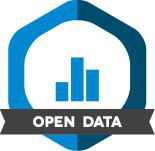
\includegraphics[width=.2\columnwidth]{OpenData}}
	\subcaptionbox{Open Materials}{
\includegraphics[width=.2\columnwidth]{OpenMaterials}}
	\subcaptionbox{Preregistered}{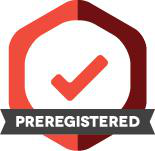
\includegraphics[width=.2\columnwidth]{Preregistered}}
	\caption{Open Science three-level badging system}\label{Fig:OpenScienceBadges}
\end{figure}

ACM -- The Association for Computing Machinery has a five-level badging system\footnote{ \url{https://www.acm.org/publications/policies/artifact-review-badging}}, illustrated in Fig.~\ref{fig:ACM-Badging}.

\begin{figure}[hbt]
	\centering
	\subcaptionbox{Functional artifacts\label{Fig:Functional}}{
\includegraphics[width=.19\columnwidth]{artifacts_evaluated_functional}}
	\subcaptionbox{Reusable artifacts\label{Fig:Reusable}}{
\includegraphics[width=.19\columnwidth]{artifacts_evaluated_reusable}}
	\subcaptionbox{Available artifacts\label{Fig:Available}}{
\includegraphics[width=.19\columnwidth]{artifacts_available}}
	\subcaptionbox{Reproducible results\label{Fig:Reproducible}}{
\includegraphics[width=.19\columnwidth]{results_reproduced}}
	\subcaptionbox{Replicable results\label{Fig:Replicable}}{
\includegraphics[width=.19\columnwidth]{results_replicated}}
	\caption{ACM five-level badging system}\label{fig:ACM-Badging}
\end{figure}

It is worth noting that levels~\ref{Fig:Functional} and~\ref{Fig:Reusable} do not grant \textit{per se} reproducibility.
They just acknowledge that the authors made their code available to reviewers, and that it is functional and reusable.
The remote sensing community should strive to attain, at least, level~\ref{Fig:Reproducible}.

We believe that a similar, even if simpler, badging system will have great positive impact in the remote sensing community.

\section{Platforms}

Konkol et al.~\cite{PublishingComputationalResearchaReviewofInfrastructuresforReproducibleandTransparentScholarlyCommunication} discuss ten infrastructures for reproducible practices.
The authors perform analyses from the viewpoints of publishers, editors, authors, readers and reviewers, and librarians.
The work is an authoritative reference for choosing among the currently available options.

In the following we will comment two different approaches, both available through IEEE.

\subsection{Code Ocean}

IEEE has teamed with Code Ocean to\footnote{\url{https://ieeexplore.ieee.org/Xplorehelp/#/faqs/code-ocean#what-is-ieee-xplore-code-ocean}}
\begin{quote}
enable authors to further enhance the visibility and impact of their research by enabling them to share their code on Code Ocean so that readers can browse, view, run and experiment with the code.

Readers can discover, browse, run, modify code, and input data to experiment, reproduce, and build on your research, all in the cloud, without any other setup or software license.
\end{quote}

Code Ocean currently supports 
C/C++, 
Fortran,
Java,
Julia,
Lua,
MATLAB,
Octave,
Perl,
Python,
R, and
Stata in most available versions.
It, thus, covers the major programming languages in which the Remote Sensing community develops its research.

The service is available to authors of already accepted papers, so it cannot be integrated into the review process.

\subsection{Data Port}

IEEE describes DataPort™ as\footnote{\url{https://ieee-dataport.org/about-ieee-dataport}} 
\begin{quote}
a valuable and easily accessible data platform that enables users to store, search, access and manage data.  
The data platform is designed to accept all formats and sizes of datasets (up to \SI{2}{\tera\byte}), and it provides both downloading capabilities and access to datasets in the Cloud.  
IEEE DataPort™ is a universally accessible web-based portal that serves four primary purposes: 
(1)~Enable individuals and institutions to indefinitely store and make datasets easily accessible to a broad set of researchers, engineers and industry;  
(2)~Enable researchers, engineers and industry to gain access to datasets that can be analyzed to advance technology;
(3)~Facilitate data analysis by enabling access to data in the AWS Cloud and by enabling the downloading of datasets
(4)~Supports reproducible research.
\end{quote}

The description concludes with a link between the technology and IEEE's mission:
\begin{quote}
IEEE DataPort™ is an online data platform created and supported by IEEE and supports IEEE’s overall mission of Advancing Technology for Humanity.  
\end{quote}
This humanitarian connection is relevant, and we consider it a cornerstone of reproducibility.
We go back to it in Section~\ref{Sec:Ownership}.


\subsection{GRSS Code Library}

The IEEE Remote Sensing Code Library -- RSCD\footnote{\url{http://www.grss-ieee.org/publication-category/rscl/}} is 
\begin{quote}
an on-line curated repository of software related to remote sensing missions, instruments, processing, and applications.

Software should be relevant to the theory, concepts, and techniques of science and engineering as applied to sensing the earth, oceans, atmosphere, and space, and the processing, interpretation, and dissemination of this information.
\end{quote}

As such, RSCD is a major player in the Remote Sensing reproducibility and replicability game.

\section{Proposal}

In this section, we propose a badging system to identify works that comply with minimum requirements of reproducibility and replicability in Remote Sensing research.
Fig.~\ref{Fig:BadgeProcess} shows the workflow for its implementation.

\subsection{Requirements}

\subsubsection{Web page}\label{Sec:WebPage}
The first requisite for being considered a RSRR is associating the manuscript to a universally accessible and informative web page containing:
\begin{enumerate}
	\item\label{item:ProjectID} Project identification (one project may host more than one paper; one paper may be hosted by more than one project)
	\begin{enumerate}
		\item Title
		\item Participants
		\item Summary
		\item Funding information
		\item Start date, state (in preparation, active, finished)
	\end{enumerate}
	\item Paper identification (if different from~\ref{item:ProjectID})
	\begin{enumerate}
		\item Title
		\item Contact: the corresponding author
		\item Abstract
		\item PDFs of relevant versions, including information of its submission to repositories (arXiv, IEEE~TechRiv, 			etc.), journal or conference
		\item\label{item:SourceDocumentFiles} \LaTeX\ and \BibTeX\ files, images, and plots
	\end{enumerate}
	\item\label{item:Platform} Computational platform (machine, model, operating system, software, libraries, and versions)
	\item Code (with comments)
	\item Data
	\item Which software components are FLOSS or free (including operating system)?
	\item Provide precise instructions and examples about:
	\begin{enumerate}
		\item How to install and run the code;
		\item How to read and modify the data;
		\item How to generate the plots, images (where they improved for visualization? how?), and tables (rounding, truncating, etc.)
	\end{enumerate}
\end{enumerate}

Most researchers are able to produce a basic web page. 
Bear in mind that basic web pages are likely to attract users, and they suffice to enrich the visibility the research.

\subsubsection{Experimental design} Many studies rely on the information provided by samples;
few of them detail the procedure with which they were collected.
A reproducible study should, besides providing the samples used, state the following:
\begin{enumerate}
	\item Objective criteria set \textit{a priori} for sample collection.
	\item Number of samples, sample size, and descriptive statistics for the aggregated data.
	\item Objective criteria for sample selection and data imputation.
\end{enumerate}

Stochastic simulation is at the core of randomized algorithms as, for instance, Monte Carlo experiments.
In order to make such algorithms reproducible, apart from the information in Section~\ref{Sec:WebPage}, item~\ref{item:Platform}, the authors must inform the pseudo-random number generator and the seeds employed.

Science is not only made of positive results.
Sticking to this path may restrict the outcomes to confirmatory studies, avoiding those lines of research that do not produce immediately publishable results.
Scientific honesty requires telling the whole story, starting from clearly defining the research protocol~\cite{TellItlikeItIs}.
The research course may change along the work, but telling the whole story adds more to the scientific knowledge that reporting only the evidence and the conclusions that are aligned with the starting hypotheses.


\subsubsection{Open data} Open data can be accessed, used, and shared by Governments, businesses and individuals. 
Open data should be stored in widely accessible and persistent repositories, in common machine-readable formats.
Please notice that Excel\textsuperscript{\textcopyright}\ spreadsheets do not comply with this requirement; use Comma-Separated Values (with \verb|.csv| extension) instead.
Although Open data are not necessarily free data, the authors must at least provide free samples.

\subsubsection{Free/Libre Open Source Software (FLOSS)}

FLOSS source code is licensed free of charge, encouraging modifications and improvements.

Notable FLOSS platforms for Remote Sensing research are 
R\footnote{\url{https://www.r-project.org/about.html}} (for statistical computing and production of high-quality graphics),
Python\footnote{\url{https://www.python.org/about/}} (an interpreted, object-oriented, high-level programming language with dynamic semantics),
GNU Octave\footnote{\url{https://booki.flossmanuals.net/command-line/gnu-octave.html#}} (an array-programming oriented language).
The European Space Agency -- ESA freely distributes SNAP -- SeNtinel’s Application Platform\footnote{\url{http://step.esa.int/main/toolboxes/snap/}}.
Developed in Java and Python.
SNAP is intended for interactive image visualisation and analysis, but it also allows scripting and software and extension with new functionalities.
Moreover, ESA promotes STEP, a community platform for accessing the software and its documentation, communicating with the developers, dialoguing within the science community, promoting results and achievements as well as providing tutorials and material for training scientists using the Toolboxes.
All platforms mentioned in this section have similar communities.

\subsubsection{Code}

Providing the code that transformed data into knowledge is a cornerstone in Remote Sensing Reproducible Research.
This requires lots of generosity, and a change of mindset, but it is fundamental for the advancement of Science.

Researchers are benefited from the assistance of well-trained programmers (software engineers) that make software's issues simpler. 
But in other situations, researchers must prepare the codes by themselves and this, is not an easy task. 
Decisions such as selecting the most appropriate tool (C?, Python?, on Windows or Linux?) or what public libraries to use are not trivial either.

Therefore, among others, software challengers related to reproducibility and replicability can be summarized as follows:
\begin{itemize}
	\item properly select the best software in terms of efficiency, to support the work;
	\item properly select the best software to be easily used, updated, and reported;
	\item make the software as easy to use as possible.
\end{itemize}

Note that software efficiency is closely related to the hardware and operating system on which it runs.
Therefore, the implementation must be designed aiming at its easy and fast adaptation to new coming machines and environments. 
This is specially true for the challengers that the deep learning paradigm brings into Remote Sensing research.

We urge authors to adhere to good practices as, for instance, those discussed in~Ref.~\cite[Chapter 7]{WritingScientificSoftware}.
Bear in mind that sharing code aims at allowing others to use it, so you must provide running examples, and comments that allow your readers to make the necessary changes for, for instance, changing the input data.

For instance, for C, Java, Python programmers, the  GNU General Public License tool, Doxygen\footnote{\url{http://doxygen.nl}}, easily generates documentation from flat sources and it also provides visual representations of the code in an hierarchical attractive and very useful way.

\subsubsection{Text}

Zobel's book~\cite{WritingforComputerScience} discusses general guidelines of adequate scientific writing.
We add elements that promote to reproducibility and replicability.

The methodological part of the text is essential for reproducibility.
It must state clearly all the assumptions, details of the context, materials, and procedures the authors employed during their research.
A good Methodology section is a roadmap for reproducing exactly the same study and, ideally, obtaining the same results.

In the same manner the authors identified missing knowledge while performing the analysis of the state-of-the art and, with it, made a contribution, their work should point at future enhancements, improvements, and advances.
The more straightforward these remarks are, the easier will be for other researchers (and for the authors themselves) to continuing contributing to this line of research.

Since the source \LaTeX\ and \BibTeX\ will be available, the authors should be generous with comments.
Such additional information will not make it to the final published work, but can be useful to those readers that will use this material.


\subsection{Implementation}

GRSS should implement a Remote Sensing Reproducibility Committee for each of its (currently) four journals, namely:
IEEE Transactions on Geoscience and Remote Sensing,
IEEE Geoscience and Remote Sensing Letters,
IEEE Geoscience and Remote Sensing Magazine, and
IEEE Journal of Selected Topics on Applied Earth Observations and Remote Sensing.
This committee will act solely on accepted papers for which the authors have requested the RSRR Badge.

The the assessment process has three possible outcomes:
\begin{itemize}
	\item \textbf{Fully RSRR:} the article is fully compliant with the reproducibility and replicability criteria.
	\item \textbf{Partially RSRR:} the article is partially compliant with the reproducibility and replicability criteria, as it does not use exclusively FLOSS software.
	\item \textbf{No badge:} the manuscript does not comply with at least one of the mandatory reproducibility requirements.
\end{itemize}

Fig.~\ref{Fig:BadgeProcess} illustrates the proposed badge awarding process.

\begin{figure}[hbt]
	\centering
	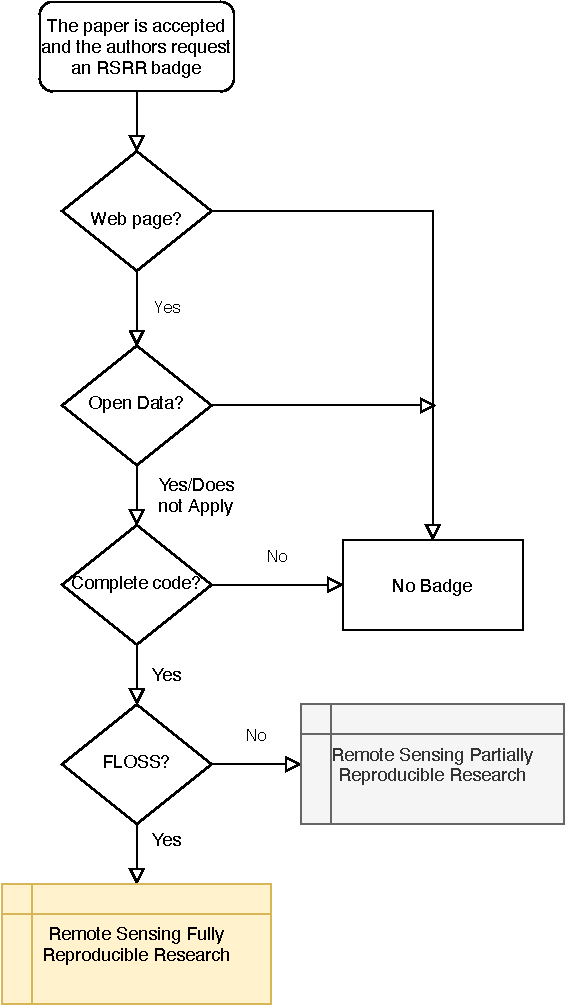
\includegraphics[width=.7\columnwidth]{BadgeAwardingProcess}
	\caption{Flowchart of the badge awarding process}\label{Fig:BadgeProcess}
	%%% The source for this figure is in /Figures/DrawIO/BadgeAwardingProcess.drawio
\end{figure}

Some of the direct benefits for papers published under the RSRR Badge are:
\begin{itemize}
	\item the paper will display the recognition (both for the paper printed and for the online versions),
	\item the paper will be specially promoted after publication by the journals,
	\item the journal will enforce, in each cross-referenced database, that the paper has that badge recognition.
\end{itemize}

The work by Santana-Cedr\'es et al~\cite{DespecklingPolSARImageswithaStructureTensorFilter2019}, for instance, qualifies for a Remote Sensing Partially Reproducible Research.

As authors' obligation, a pre-requisite to obtain the badge is the acknowledgement that the paper is reproducible in all the terms for a period of at least five years, and that the material has permanent and global identifiers, e.g., DOIs.

\section{Tools}

Starting well saves lots of time.
We make recommendations that may save time and efforts.
All of them are either free, or offer a free operational version which usually suits the needs of relatively small remote sensing reproducible research projects.

\subsection{Doodling}

Doodling is an important stage to unlock creativity in a controlled manner.
We suggest using FreeMind\footnote{\url{http://freemind.sourceforge.net/wiki/index.php/Main_Page}}, or any other mind map tool, for this purpose.

Figure~\ref{Fig:Doodle} shows the mind map product of such doodling stage.
It served as guide for the structure of this paper.

\begin{figure}[hbt]
\centering
\includegraphics[width=\linewidth]{"Badging RSRR.pdf"}
\caption{The mind map that led to this paper.}\label{Fig:Doodle}
%%% The source is in /Figures/FreeMind/Badging RSRR.mm
\end{figure}

Having such an editable visual structure, along with properties and relationships between elements, helps reminding and documenting the progress of the project.

\subsection{Git repository}

We assume in this section that you use \LaTeX\ and \BibTeX.

The main idea consists in having a single repository for all the scientific texts you write: 
theses, 
reports, 
articles, 
letters,
reviews,
and miscellaneous documents.

Fig.~\ref{Fig:StructRepo} illustrates the recommended basic structure for a repository holding several \LaTeX\ files (or projects), along with their associated data and code.

\begin{figure}[hbt]
	\centering
	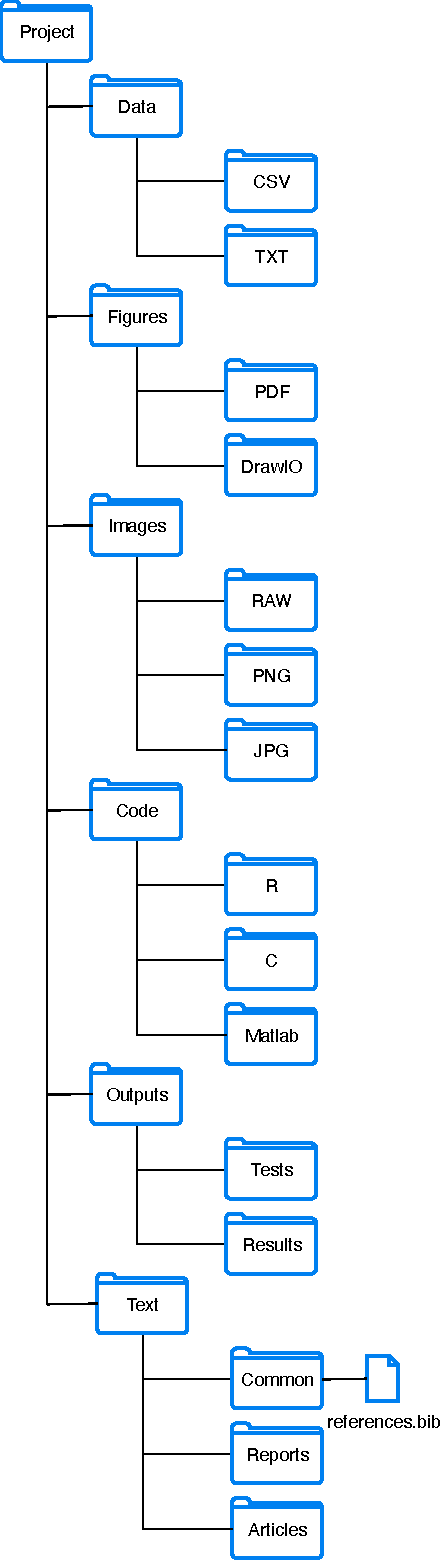
\includegraphics[width=.35\columnwidth]{DirectoryStructure}
	\caption{Recommended structure of a repository for scientific projects.}\label{Fig:StructRepo}
	%%% The source is in /Figures/DrawIO/DirectoryStructure.drawio
\end{figure}

Every directory may contain specific subdirectories.
For instance, \verb|Data| may contain \verb|CSV|, \verb|text|, and other directories with specific data files.

Notice that there is a single \BibTeX\ file (with extension \verb|.bib| in the \verb|Common| directory).
\BibTeX\ references can be split on several files, but these files should be common to all projects.
This avoids outdated and redundant bibliographic data bases.

Every article should be in its own directory.
Avoid using the name of the journal where you will submit your work for the directory and document names, as the destination may change along the process.

Data, figures, images and code should be common to all projects, as one typically reuses them.
Inform in your \LaTeX\ code the source of each figure, for instance with a comment of the form \texttt{\%\%\% The source is in ../../Figures/DrawIO/DirectoryStructure.drawio}.
This will help the review process, and the communication between authors. 
All references to source files must use relative paths, e.g., \texttt{../../more-path/figures}, and \texttt{../../more-path/video\_demos}. 
This applies also to codes (\texttt{../../more-path/my\_personal\_library}).


The \verb|Outputs| directory should contain both intermediate, but interesting, results (in \verb|Tests|), and those results that made it into the final report (in \verb|Results|).
Good documentation is fundamental to help you, your team, and others to catch up from where you stopped.	

Check Ref.~\cite{EditorialGRSL2015} for a naming convention and suggestions for revision handling of submitted manuscripts.

\subsection{Communication}

Most of the research in remote sensing is collaborative, and involves two or more authors.
This is mostly due to the interdisciplinary nature of the area, which requires complementary competencies.
Communication in such scenario is of paramount importance.

Although e-mail is a powerful tool, synchronous communication is often required.
WhatsApp and WeChat are the commonplace for real-time exchange of ideas, but they do not offer either the tools or the organization required for prolific and time-saving technical conversations.

Slack\footnote{\url{https://slack.com/}} serves this purpose well.
It organizes conversations in channels, connects with other applications (Google Suit, meetings, Github, polls, etc.) promoting, thus, focus and persistence.

\subsection{Task management}

We have stressed the importance of using a Kanban-style management method for building a project~\cite{SuccessfulScientificPublishingfromtheProjecttotheAdvertising}.
Such method is also recommended for simple task management.
Trello\footnote{\url{https://trello.com/}} usually meets well the needs of organizing and maintaining a Remote Sensing reproducible project, but a more sophisticated tool, such as ProjectLibre\footnote{\url{https://www.projectlibre.com/}} is highly advisable for projects which involve several participants, resources, deliverables, and deadlines.

Fig.~\ref{Fig:ScientificCanvas} shows the structure of a Scientific Canvas in Trello, freely available at \url{https://trello.com/b/C747M1GX}.
Cards are organized in lists, and lists in groups.
This board can be copied, and assigned to a team, whose leader can assign tasks (cards), with deadlines, reminders, and several other utilities.
Details of such organization, which is inspired by the canvases discussed in Ref.~\cite{osterwalder2010business}, were presented in~\cite{SuccessfulScientificPublishingfromtheProjecttotheAdvertising}.

\begin{figure}[hbt]
\centering
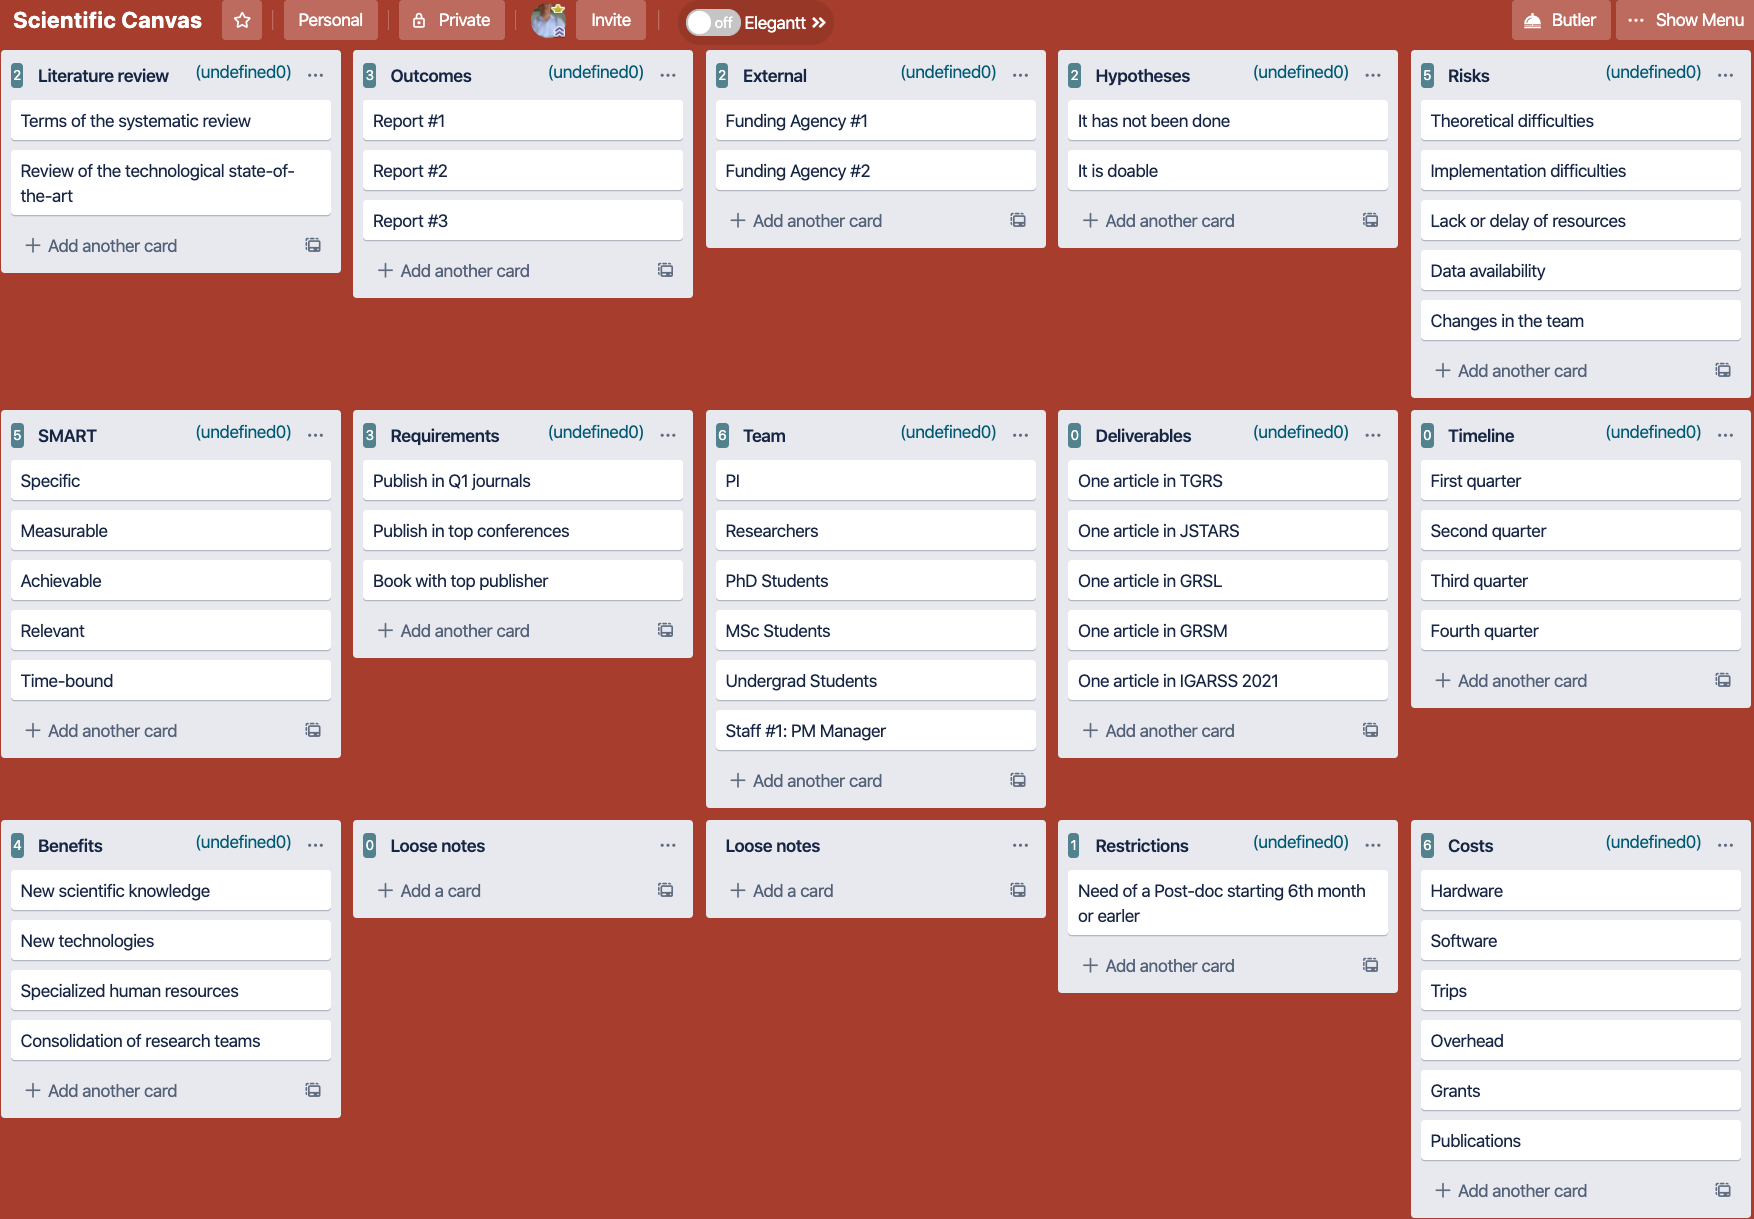
\includegraphics[width=\linewidth]{ScientificCanvas}
\caption{A Trello implementation of a Scientific Canvas}\label{Fig:ScientificCanvas}
\end{figure}

As Trello keeps track of every single modification, it becomes a useful resource when it comes to reproducibility.

\section{Challenges}

\subsection{Point-and-click software}

The ease of use of point-and-click software based on predefined menus is undeniable.
Such platforms may conspire against reproducibility, though.
A fully reproducible process, if totally based on such a platform, must state step-by-step the procedure.
For this reason, it is advisable to prefer software that allows coding.

\subsection{Machine Learning}

Machine learning in general, and CNNs -- Convolutional Neural Networks in particular, have seen lately an extraordinary increase in popularity in the Remote Sensing community~\cite{DeepLearningandProcessUnderstandingforDataDrivenEarthSystemScience}. 
Any reproducible approach must pay special attention to what this so efficient machine learning approach is capable to get from data (specially from the Big Data).
Isdahl and Gundersen~\cite{OutoftheBoxReproducibilityaSurveyofMachineLearningPlatforms}

Some of the challenges that these studies pose for their reproducibility are random initialization, and the need of GPU resources. 

\subsection{Culture}

\subsubsection{Overhead}

Most experienced researchers frown upon adhering to new practices, specially if they are already successful.
It is worth noting that many scientific practices are changing, and adaptation is a sign of intelligence, if not requirement for survival.

The learning curve of good reproducibility and replicability practices is not steep, and they can be adopted gradually.
We have noticed that students and young researchers may be the drivers of this change which, once in place, facilitates high quality research.

We, thus, consider that overhead is small, limited to the initial stage of the adoption of the practices, and that it returns in the form of better recognition and smoother work.

\subsubsection{Ownership}\label{Sec:Ownership}

The Universal Declaration of Human Rights\footnote{\url{https://www.un.org/en/universal-declaration-human-rights/}}, in its Article 27, states that
\begin{quotation}
	Everyone has the right freely to participate in the cultural life of the community, to enjoy the arts and to share in scientific advancement and its benefits.
\end{quotation}




	
\section*{Acknowledgments}

The authors would like to thank CNPq and Fapeal (Brazil) for partial support of this work.
	
%\nocite{StatisticalAnalysesReproducibleResearch,%
%RRComputationalHarmonicAnalysis,%
%RREconometrics,%
%RRSignalProcessing,%
%AddressingNeedDataCodeSharingComputationalScience,%
%ReproducibleResearchinComputationalScience,%
%TenRulesReproducibleComputationalResearch,%
%AddressingNeedDataCodeSharingComputationalScience,
%SevenReasonsWhyaUsersGuidetoTransparencyandReproducibility,%
%OutoftheBoxReproducibilityaSurveyofMachineLearningPlatforms,%
%ReproducibilityofScientificResults2018,%
%ReproducibleResearchandGIScienceanEvaluationUsingAGILEConferencePapers,%
%TheStateofReproducibilityintheComputationalGeosciences}
	
\bibliographystyle{IEEEtran}
\bibliography{../../Common/references}

	
\end{document}



